\documentclass[
    10pt,
    aspectratio=169,
    xcolor={dvipsnames},
    spanish,
    % handout,
    % notes=only,
    % notes,
    ]{beamer}

% BEAMER SETTINGS
\setbeamerfont{section in toc}{size=\normalsize, shape=\bfseries}
\mode<presentation>{
    \usetheme{Antibes}
    \setbeamercovered{transparent}
    \usecolortheme{rose}
    \setbeamertemplate{navigation symbols}{}
    }
\useoutertheme{infolines}

% PACKAGES
% \usepackage[spanish]{babel}  % uncomment for Spanish support
\usepackage{tikz,pgfplots}
\pgfplotsset{compat=1.13}
\usetikzlibrary{calc}
\usepackage{subcaption}
\usepackage{graphicx}
\graphicspath{{figures}}
\usepackage{booktabs}
\usepackage{upgreek}
\usepackage{commath}
\usepackage{amsmath,amsthm,amssymb,mathtools,mathrsfs}
\usepackage{cancel}
\usepackage{fontawesome5}
\usepackage{enumerate}
\usepackage{tensor}
\usepackage[font=footnotesize]{caption}
\usepackage{wasysym}
\usepackage{wrapfig}
\usepackage[skins,theorems]{tcolorbox}
\tcbset{
    highlight math style={
        enhanced,
        coltext=black,
        colframe=black,
        colback=lightgray,
        arc=0pt,
        boxrule=.5pt
        }
}

% REFERENCES AND OTHERS
\usepackage{aas_macros}
\usepackage{natbib}
\bibpunct{(}{)}{;}{a}{}{,}

\usepackage{siunitx}
\sisetup{
    range-phrase=\text{--},
    range-units=single,
    separate-uncertainty=true,
    print-unity-mantissa=false
    }
\DeclareSIUnit{\gauss}{G}
\DeclareSIUnit{\jansky}{Jy}
\renewcommand{\figurename}{Fig.}

\usepackage{hyperref}
\hypersetup{
    % bookmarks=true,
    unicode=true,
    pdftoolbar=true,
    pdfmenubar=true,
    pdffitwindow=false,
    pdfstartview={FitH},
    pdftitle={CHART LPDA design},
    pdfauthor={Erik Saez A.},
    pdfcreator={Erik Saez A.},
    pdfnewwindow=true,
    colorlinks=true,
    linkcolor=RoyalBlue,
    citecolor=RoyalBlue,
    urlcolor=RoyalBlue
    }

\title[Presentation practice II]{\bfseries Auxiliar 7}
\subtitle{Energías Renovables No Convencionales}
\author[Erik Saez A.]{Erik Saez A.}
\institute[UChile]{Department of Electrical Engineering \\ Universidad de Chile}
\date{\today}
\begin{document}
\begin{frame}
  \titlepage
  \centering
  \faIcon{envelope} \href{mailto:erik.saez@ug.uchile.cl}{erik.saez@ug.uchile.cl} \hspace{.2cm}
\end{frame}

\begin{frame}
  \frametitle{Contents}
  \centering
  \begin{columns}
    \begin{column}{0.4\textwidth}
      \tableofcontents
    \end{column}
    \begin{column}{0.5\textwidth}
      \begin{figure}
        \centering
        
\includegraphics[width=\textwidth]{fcfm_die}
        \caption{Facultad de Ciencias Físicas y Matemáticas , Universidad de Chile.}
      \end{figure}
    \end{column}
  \end{columns}  
\end{frame}
%------------------------------------------------
%Resumen
%------------------------------------------------
\section{Resumen}
%------------------------------------------------
%Preguntas conceptuales
\section{Preguntas conceptuales}
%------------------------------------------------
\begin{frame}{Preguntas conceptual}
\begin{block}{Ejemplo de pregunta conceptual 1}
  ¿Cuál es la principal diferencia en los componentes utilizados entre las centrales generadoras convencionales y las centrales basadas en ERNC? Explica cómo esta diferencia afecta los sistemas de control utilizados en cada tipo de central.
\end{block}
\end{frame}
%-------------------------------------------------
\begin{frame}
\begin{block}{Solucion de pregunta conceptual 1}
  ¿Cuál es la principal diferencia en los componentes utilizados entre las centrales generadoras convencionales y las centrales basadas en ERNC? Explica cómo esta diferencia afecta los sistemas de control utilizados en cada tipo de central.
\end{block}
\textbf{Solución:} Las centrales convencionales suelen estar basadas en generadores sincrónicos, los cuales convierten la energía mecánica de un fluido (como gas o agua) en energía eléctrica. Estas centrales generalmente cuentan con una turbina y un generador eléctrico sincrónico. Por otro lado, las centrales basadas en ERNC dependen más de la electrónica de potencia y pueden incluir convertidores estáticos, generadores de inducción y sincrónicos, además de sistemas de almacenamiento como baterías. Esta diferencia en componentes implica que las centrales ERNC requieren sistemas de control más complejos para gestionar la conversión de energía de fuentes variables, como el sol o el viento.
\end{frame}
%-------------------------------------------------
\begin{frame}
\begin{block}{Ejemplo de pregunta conceptual 2}
  Explica cómo se genera la potencia en un aerogenerador y describe el rol de la velocidad del viento en la curva de potencia, incluyendo las velocidades de \textit{Cut-in} y \textit{Cut-out}.
\end{block}
\begin{figure}
  \centering
  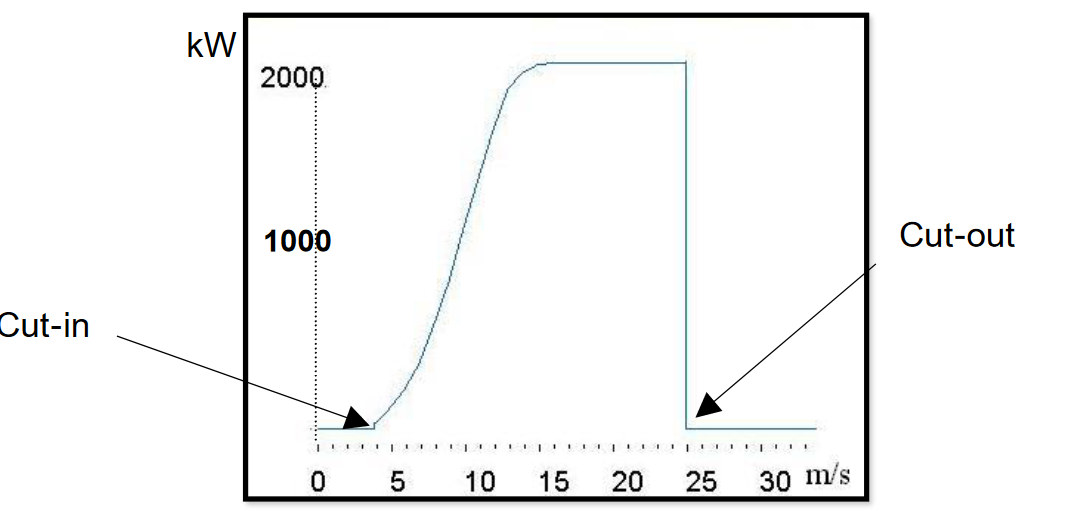
\includegraphics[width=0.5\textwidth]{Figure_1.png}
  \caption{Curva de potencia de un aerogenerador}
\end{figure}
\end{frame}
%-------------------------------------------------
\begin{frame}
  \begin{block}{Ejemplo de pregunta conceptual 2}
    Explica cómo se genera la potencia en un aerogenerador y describe el rol de la velocidad del viento en la curva de potencia, incluyendo las velocidades de \textit{Cut-in} y \textit{Cut-out}.
  \end{block}
\textbf{Solución:} La potencia generada en un aerogenerador se calcula utilizando la ecuación 
\[
P_{\text{eléctrica}} = \frac{1}{2} C_p C_m C_e \rho v^3 A,
\]
donde \( C_p \), \( C_m \) y \( C_e \) son coeficientes que dependen de la eficiencia del sistema, \( \rho \) es la densidad del aire, \( v \) es la velocidad del viento, y \( A \) es el área barrida por las palas. La velocidad del viento afecta directamente la potencia generada. La velocidad de ``Cut-in'' es la mínima velocidad del viento necesaria para que el aerogenerador comience a generar potencia. Al alcanzar la velocidad de ``Cut-out'', el aerogenerador se apaga para evitar daños estructurales por vientos excesivamente fuertes.
\end{frame}
%-------------------------------------------------
\begin{frame}
  \begin{block}{Ejemplo de pregunta conceptual 3}
    ¿Qué es la ley de Betz y cuál es su implicancia en la eficiencia máxima teórica de un aerogenerador?
  \end{block}
  \begin{figure}
    \centering
    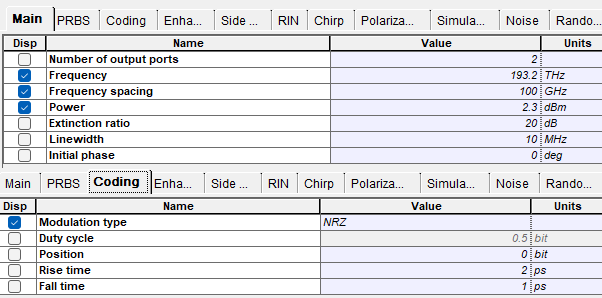
\includegraphics[width=0.5\textwidth]{Figure_2.png}
    \caption{Grafico de potencia en relacion a la ley de Betz}
  \end{figure}
\end{frame}
%-------------------------------------------------
\begin{frame}
  \begin{block}{Ejemplo de pregunta conceptual 3}
    ¿Qué es la ley de Betz y cuál es su implicancia en la eficiencia máxima teórica de un aerogenerador?
  \end{block}
\textbf{Solución:} La ley de Betz establece que la eficiencia máxima teórica de un aerogenerador para convertir la energía cinética del viento en energía mecánica es del 59\%. Esto significa que, en condiciones ideales, solo se puede aprovechar un 59\% de la potencia del viento que atraviesa el área barrida por las palas. Este límite se debe a que no toda la energía del viento puede ser capturada; una parte debe permanecer en el flujo de aire para que el viento continúe moviéndose a través de las palas.
\end{frame}
%-------------------------------------------------
\begin{frame}
  \begin{block}{Ejemplo de pregunta conceptual 4}
    Describe los tipos de aerogeneradores de eje horizontal y de eje vertical, y menciona una ventaja y una desventaja de cada uno.
  \end{block}
\end{frame}
%-------------------------------------------------
\begin{frame}
  \begin{block}{Ejemplo de pregunta conceptual 4}
    Describe los tipos de aerogeneradores de eje horizontal y de eje vertical, y menciona una ventaja y una desventaja de cada uno.
  \end{block}
\textbf{Solución:} Los aerogeneradores de \textit{eje horizontal} son los más utilizados para la generación eléctrica a gran escala, ya que se acercan más a los límites teóricos de aprovechamiento de la energía del viento. Una ventaja es que permiten un uso eficiente del recurso viento, mientras que una desventaja es que son más sensibles a variaciones de tensión. Por otro lado, los aerogeneradores de \textit{eje vertical} se utilizan en aplicaciones de baja escala o en condiciones de alta solidez, como molienda o bombeo. Una ventaja de este tipo es su estructura robusta, que soporta mejor las fluctuaciones de velocidad del viento, pero tienen una menor eficiencia en la conversión de energía en comparación con los aerogeneradores de eje horizontal.
\end{frame}
%-------------------------------------------------
\section{Pregunta 2}
  \begin{frame}{Pregunta 2}
    \begin{block}{Enunciado Pregunta 2}
      Considerando los datos de la siguiente tabla, construya las curvas V-I y V-P para el panel fotovoltaico para las siguientes condiciones (indicando los MPP's de cada uno):

      \begin{table}[h!]
        \scriptsize
          \centering
          \begin{tabular}{|c|c|}
              \hline
              \textbf{Parámetro} & \textbf{Valor} \\
              \hline
              $I_{sc}$ & 15 [A] \\
              $V_{oc}$ & 70 [V] \\
              $K_i$ & 0,0032 [A/K] \\
              $K_v$ & -0,123 [V/K] \\
              $\alpha$ & 1,3 \\
              $R_s$ & 0,221 [$\Omega$] \\
              $R_p$ & 415,405 [$\Omega$] \\
              $N_s$ & 30 \\
              \hline
          \end{tabular}
      \end{table}
      
      \begin{enumerate}
          \item Condiciones estándar (1000 W/m$^2$ y 25 [ºC])
          \item $G = 1000$ W/m$^2$ y $T = 10$[ºC]
          \item $G = 500$ W/m$^2$ y $T = 25$[ºC]
      \end{enumerate}
      
      Comente los resultados, ¿Tiene sentido lo obtenido?      
  \end{block}
\end{frame}

%-------------------------------------------------
\begin{frame}
  \begin{block}{Resolución pregunta 2}
    \footnotesize 
      \begin{itemize}
        \item Primero, notar que las curvas V-I son una ecuación del tipo implícita, ya que no es directo despejar \( i \) en función de \( v \).
        \item Lo anterior amerita el uso de una función que resuelva expresiones de tipo \( f(v, i) = 0 \), iterando sobre un vector de tensiones dado.
      \end{itemize}
      La ecuación de corriente es la siguiente:
      \begin{figure}
        \centering
        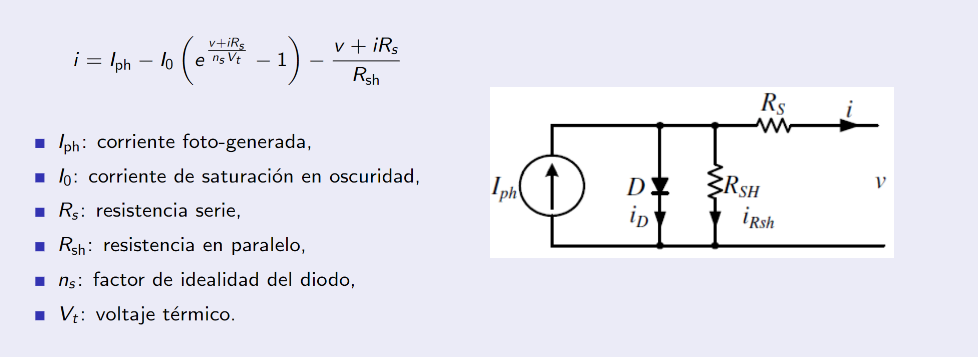
\includegraphics[width=0.8\textwidth]{Figure_3.png}
        \caption{Elementos de un panel fotovoltaico y ecuación de corriente.}
      \end{figure}
  \end{block}
\end{frame}
%-------------------------------------------------
\begin{frame}{Implementacion en Matlab}
  \begin{block}{Guardar las variables}
    Lo primero sera guardar las diferentes constantes del panel fotovoltaico ademas de las constantes de q y k que seran utilizadas para obtener $v_{T}$.
\begin{figure}
  \centering
  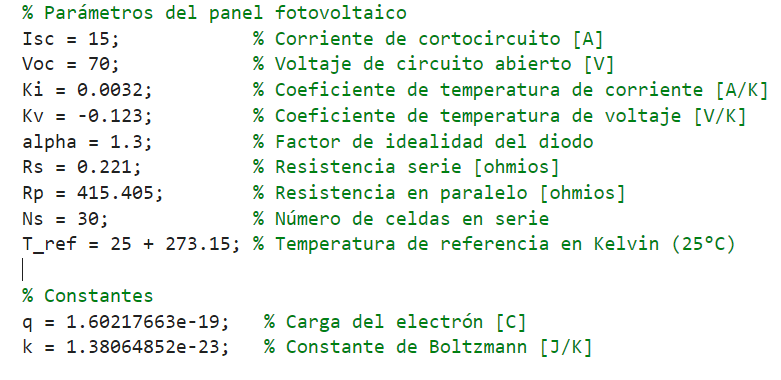
\includegraphics[width=0.5\textwidth]{Figure_4.png}
\end{figure}
\end{block}
\end{frame}
%-------------------------------------------------
\begin{frame}
  \begin{block}{Funcion en Matlab}
    luego se busca implementar la funcion que permita obtener la corriente en funcion de la tension, para ello se implementa la siguiente funcion en Matlab.
\begin{figure}
  \centering
  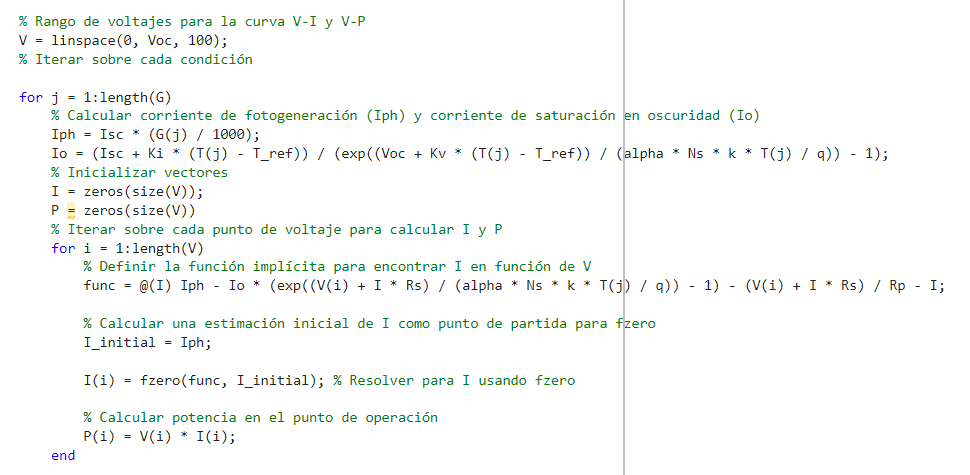
\includegraphics[width=0.65\textwidth]{Figure_5.png}
\end{figure}
\end{block}
\end{frame}
%-------------------------------------------------
\begin{frame}
  \begin{block}{Obtencion de la curva de corriente en funcion de la tension}
    Luego de implementar la funcion, se procede a graficar la curva de corriente en funcion de la tension para las diferentes condiciones dadas.
    \begin{figure}
      \centering
      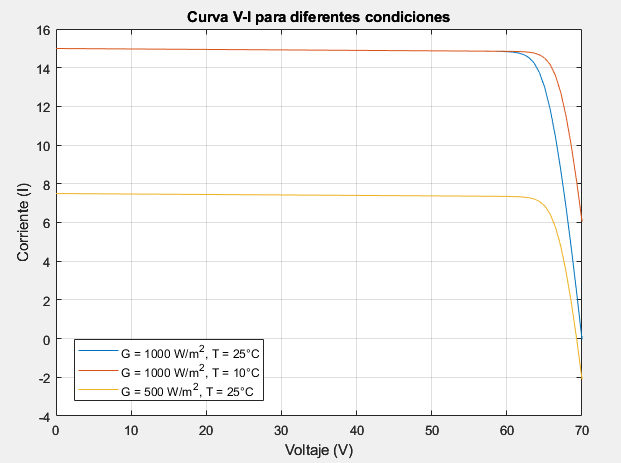
\includegraphics[width=0.5\textwidth]{Figure_6.png}
      \caption{Curva de corriente en funcion de la tension para las diferentes condiciones dadas.}
    \end{figure}
  \end{block}
\end{frame}
%-------------------------------------------------
\begin{frame}
  \begin{block}{Obtencion de la curva de la potencia en funcion de la tension}
    Se procede a graficar la curva de potencia en funcion de la tension para las diferentes condiciones dadas.
    \begin{figure}
      \centering
      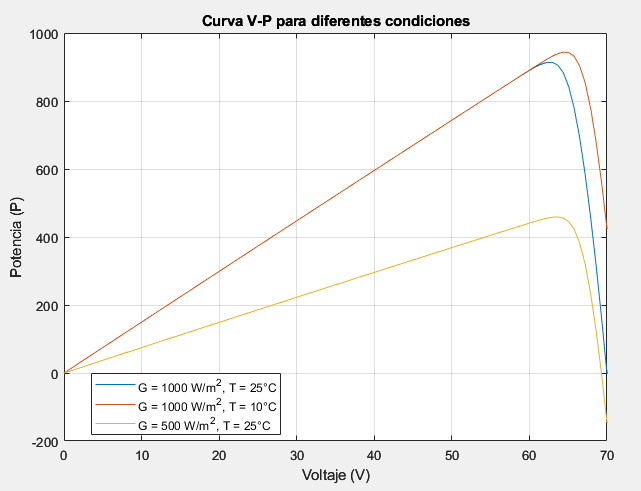
\includegraphics[width=0.5\textwidth]{Figure_7.png}
      \caption{Curva de potencia en funcion de la tension para las diferentes condiciones dadas.}
    \end{figure}
  \end{block}
\end{frame}
%-------------------------------------------------
\begin{frame}
  \footnotesize
  \begin{block}{Conclusiones}
    Estos resultados tienen sentido, ya que la generación de energía en un panel fotovoltaico depende directamente de la irradiancia (cantidad de luz solar) y de la temperatura. Una mayor irradiancia incrementa la corriente generada, mientras que una menor temperatura favorece un mayor voltaje de circuito abierto, mejorando la eficiencia. Este comportamiento es consistente con las propiedades físicas de los materiales semiconductores utilizados en las celdas solares.
    \begin{figure}
      \centering
      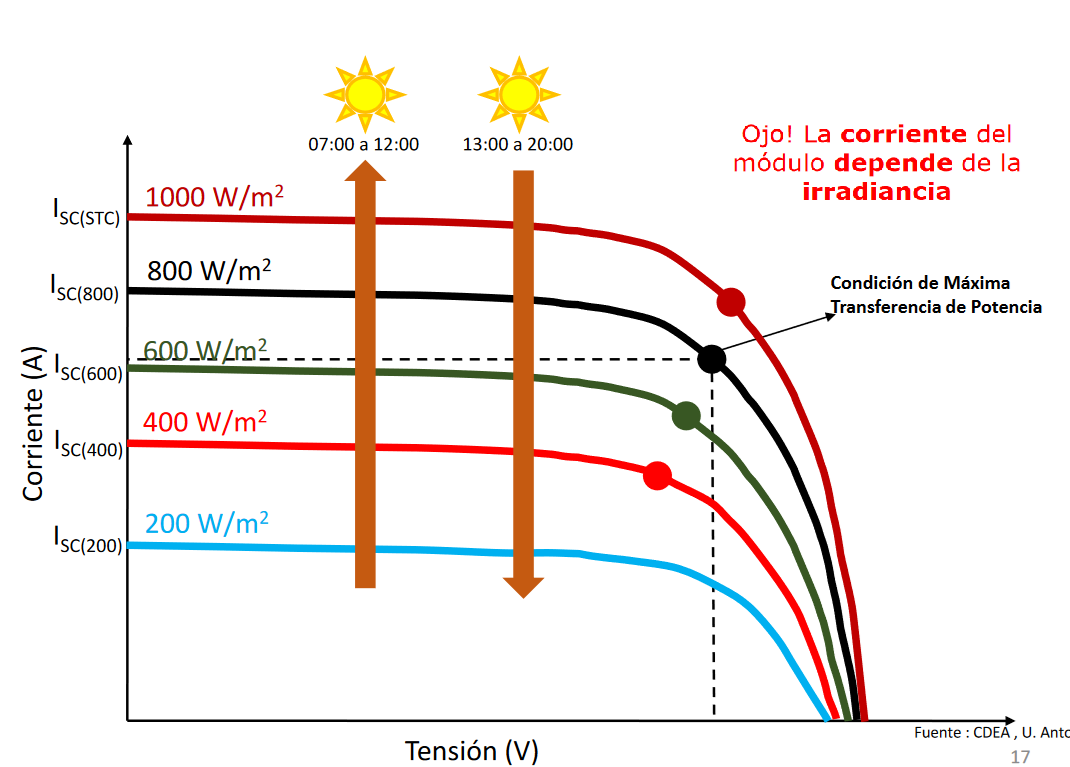
\includegraphics[width=0.4\textwidth]{Figure_8.png}
      \caption{Curvas I-V de un módulo fotovoltaico para diferentes niveles de irradiancia, mostrando que la corriente generada depende directamente de la irradiancia. El punto de máxima potencia varía con la irradiancia, optimizando la generación de energía.}
    \end{figure}
  \end{block}  
\end{frame}
%-------------------------------------------------
\section{Pregunta 3}
%-------------------------------------------------
\begin{frame}{Pregunta 3}
\begin{block}{Enunciado Pregunta 3}
  Una turbina eólica está acoplada a un generador de inducción trifásico de 560 kW, 50 Hz y 4 polos. La turbina tiene 47 metros de diámetro, una velocidad del viento nominal de 11 [m/s] y una caja de amplificación de velocidad de relación 1:52,6514.
  Considere el siguiente coeficiente de desempeño:
  \[
  C_p(\lambda) = 0.0013 \lambda^3 - 0.0439 \lambda^2 + 0.4083 \lambda - 0.6703
  \]
  \begin{enumerate}
      \item Grafique el coeficiente de desempeño \( C_p \) en función de \( \lambda \).
      
      \item Suponiendo que la turbina funciona acoplada a un generador de velocidad fija (con deslizamiento de -3\%), grafique la potencia bruta (antes de \( C_p \)) y potencia obtenida desde la turbina (considerando \( C_p \)) para velocidades del viento entre cero y velocidad nominal. ¿Cuál es la velocidad de cut-in para este modo de funcionamiento?
      
      \item Para el caso anterior, grafique la curva de potencia considerando la velocidad de cut-in determinada, una potencia máxima a velocidad nominal y una velocidad cut-out de \( v = 25 \, \text{m/s} \).
  \end{enumerate}
  
\end{block}
\end{frame}
%-------------------------------------------------
\begin{frame}
  \begin{block}{Resolucion Pregunta 3}
  Se grafica el coeficiente de desempeño \( C_p \) en función de \( \lambda \) para la función dada.
  \begin{figure}
    \centering
    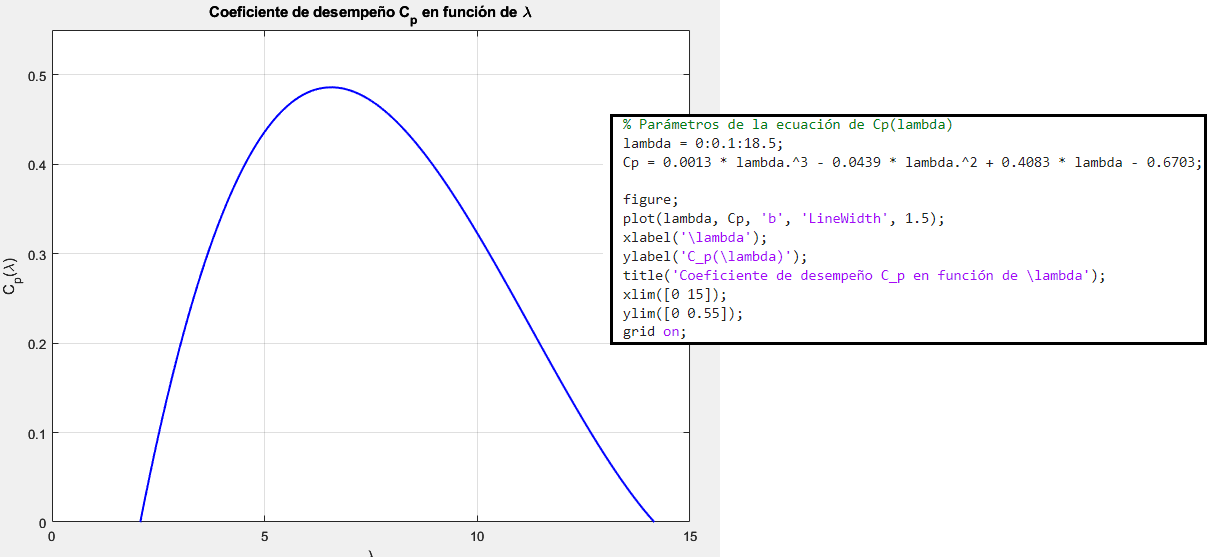
\includegraphics[width=0.7\textwidth]{Figure_9.png}
    \caption{Grafico de \( C_p \) en función de \( \lambda \).}
  \end{figure}
\end{block}
\end{frame}
%-------------------------------------------------
\begin{frame}
  \begin{block}{Resolucion Pregunta 3}
     Se procede a graficar la potencia bruta y la potencia obtenida desde la turbina para velocidades del viento entre cero y velocidad nominal. Para lo cual se consideran las ecuaciones:
    \begin{align}
      P_{\text{bruta}} &= \frac{1}{2} \rho A v^3, \\
      P_{\text{turbina}} &= P_{\text{bruta}} C_p(\lambda),
    \end{align}
    Donde tenemos que \( \lambda = \frac{v D}{N_s} \), con \( D \) el diámetro de la turbina y \( N_s \) el número de polos.
  \end{block}
\end{frame}
%-------------------------------------------------
\begin{frame}
  \footnotesize
  \begin{alertblock}{Consideracion}
    \begin{itemize}
      \item Es importante el destacar que hasta aprxoimadamente 3 m/s la potencia en la turbina es mayor a la incidcente, lo cual no tiene sentido y por tanto se asume que en dicho tramo no existe potencia.
      \item  Si se observa con detención, se puede notar que a partir de v=5.1 m/s la potencia empieza a crecer continuamente. Por lo anterior, se define $v_cut_in$ = 5.1
    \end{itemize}
  \end{alertblock}
  \begin{block}{Resolucion Pregunta 3}
    \begin{figure}
      \centering
      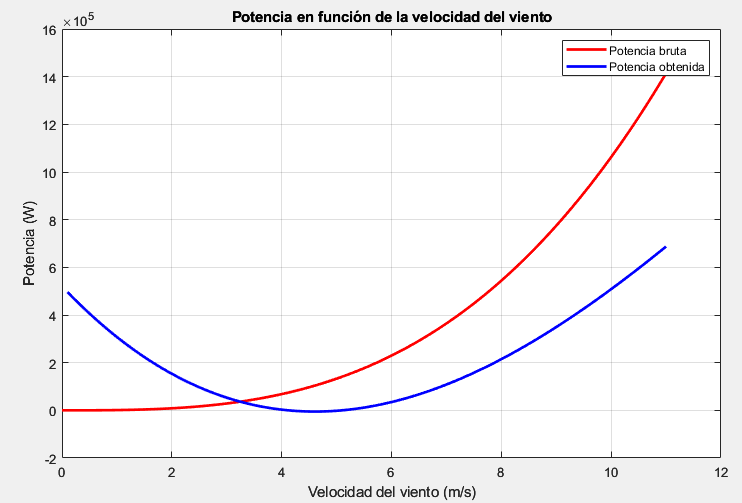
\includegraphics[width=0.4\textwidth]{Figure_10.png}
      \caption{Grafico de la potencia bruta y la potencia obtenida desde la turbina para velocidades del viento entre cero y velocidad nominal.}
    \end{figure}
  \end{block}
\end{frame}
%-------------------------------------------------
\begin{frame}
  \begin{block}{Resolucion Pregunta 3}
    Se procede a graficar la curva de potencia considerando la velocidad de cut-in determinada, una potencia máxima a velocidad nominal y una velocidad cut-out de \( v = 25 \, \text{m/s} \).
    \begin{figure}
      \centering
      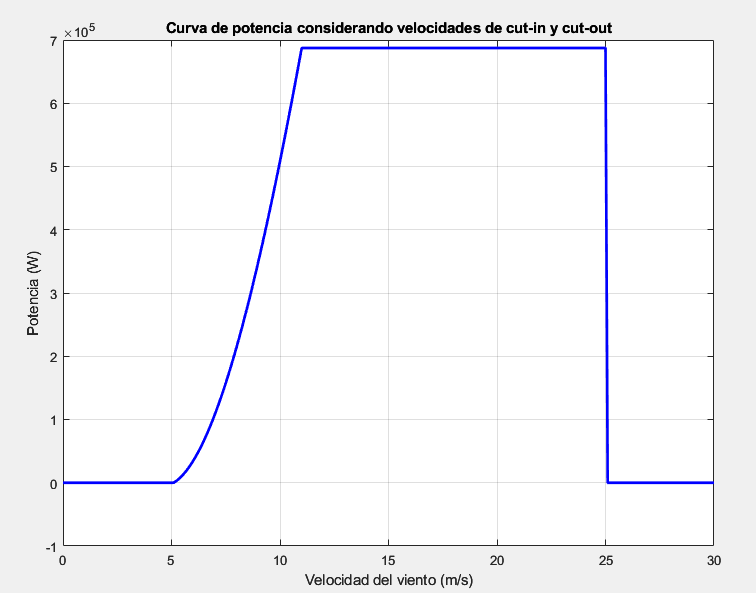
\includegraphics[width=0.4\textwidth]{Figure_11.png}
      \caption{Curva de potencia considerando la velocidad de cut-in determinada, una potencia máxima a velocidad nominal y una velocidad cut-out de \( v = 25 \, \text{m/s} \).}
    \end{figure}
  \end{block}
\end{frame}
%-------------------------------------------------
\end{document}